\documentclass[10pt,a4paper]{article}

%double si on veut une version prof et une version élève. simple si on veut une seule version.
\newcommand{\buildmode}{simple}

\InputIfFileExists{version.tex}{}{}
% Version (définie par le script)
\providecommand{\version}{eleve}

\usepackage{feuillecorrection}

%%%à modifier à chaque fois

\renewcommand{\niveau}{2nde}
\renewcommand{\chapitre}{Révisions}
\renewcommand{\numchap}{2 à 4}
\renewcommand{\theme}{Travail en distanciel}

%%% Axe gradué de -5 à 5 (graduations au quart) ; #1 : points à placer (code TikZ)
\newcommand{\axeplace}[1]{
\begin{center}
\begin{tikzpicture}[scale=1.4]
\draw[->] (-5.5,0)--(5.5,0);
\foreach \x in {-5,..., 4}{
    \draw (\x,0.1)--(\x,-0.1) node[below] {\(\x\)};
    \draw (\x+0.5,0.07)--(\x+0.5,-0.07) ;
    \foreach \minx in {0.25, 0.5, 0.75}{
        \draw (\x+\minx, 0.05)--(\x+\minx, -0.05);
    }
}
    \draw (5,0.1)--(5,-0.1) node[below] {\(5\)};
#1
\end{tikzpicture}
\end{center}
}

\begin{document}

\montitre{Révisions des premiers chapitres -- Correction}

%%%%%%%%%%%%%%%%%%%%%%%%%%%%%%%%%%%%%%%%%%%%%%%%%%%%%%%%%%%%%%%%%%%%%%%%%%%%%
\section{Proportions, pourcentages}

\begin{corr}[Calculs de début de cours]{1}
\begin{enumerate}[leftmargin=*]
    \item \begin{tasks}(3)
        \task \(3-4=-1\)
        \task \(4-3=1\)
        \task \(-3+4=1\)
        \task \(3-(-5)=3+5=8\)
        \task \(-2+7-4=1\)
        \task \(-8-(-3)=-8+3=-5\)
    \end{tasks}
    \item \begin{tasks}(4)
        \task \(1x=x\)
        \task \(0x=0\)
        \task \(-1x=-x\)
        \task \(3x-2x=x\)
    \end{tasks}
    \item Pour \(x=2\) : \(3\times 2-7=6-7=-1\). \qquad Pour \(x=-1\) : \(3\times(-1)-7=-3-7=-10\).
\end{enumerate}
\end{corr}

\begin{corr}[Guidé]{2}
\begin{enumerate}[leftmargin=*]
    \item \(p=\dfrac{8}{32}=\dfrac{1\times 8}{4\times 8}=\dfrac{1}{4}\).
    \item \(\dfrac{1}{4}=0,25=25\,\%\).
    \item On passe de \(25\) à \(100\) en multipliant par \(4\) : \(7\times 4=28\). La proportion est donc \(\dfrac{28}{100}=28\,\%\).
    \item \(28\,\%>25\,\%\) : la proportion d'élèves venant à vélo est plus grande dans la seconde classe, alors que l'effectif d'élèves venant à vélo y est plus petit (\(7<8\)).
\end{enumerate}
\end{corr}

\begin{corr}{3}
\begin{tasks}(4)
    \task \(120\)
    \task \(7\)
    \task \(15\)
    \task \(30\)
    \task \(9\)
    \task \(4,5\)
    \task \(9\)
    \task \(10\)
\end{tasks}
Par exemple : \(25\,\%\) de \(60\), c'est le quart de \(60\), soit \(15\). Pour le dernier calcul, \(20\,\%\) de \(500\) vaut \(100\), puis \(10\,\%\) de \(100\) vaut \(10\).
\end{corr}

\begin{corr}{4}
\begin{enumerate}[leftmargin=*]
    \item \(\dfrac{12}{50}=\dfrac{6}{25}=0,24=24\,\%\).
    \item \(\dfrac{30}{200}=\dfrac{3}{20}=0,15=15\,\%\).
    \item \(\dfrac{9}{20}=0,45=45\,\%\).
\end{enumerate}
\end{corr}

\begin{corr}{5}
\begin{enumerate}[leftmargin=*]
    \item \(n=p\times N=0,35\times 60\,000=21\,000\) : \(21\,000\) spectateurs sont venus en RER.
    \item \(N=\dfrac{n}{p}=\dfrac{18\,000}{0,4}=45\,000\) : il y avait \(45\,000\) spectateurs.
    \item \(p=\dfrac{13\,500}{54\,000}=0,25=25\,\%\).
\end{enumerate}

\begin{rappel}
Avec un tableau de proportionnalité (question 2) :
\begin{center}
\renewcommand{\arraystretch}{1.5}
\begin{tabular}{|l|c|c|}
    \hline
    Spectateurs venus en RER & \(40\) & \(18\,000\) \\ \hline
    Effectif total & \(100\) & \(\dots\) \\ \hline
\end{tabular}
\end{center}
\(18\,000\times 100\div 40=45\,000\).
\end{rappel}
\end{corr}

\begin{corr}[QCM]{6}
\begin{enumerate}[leftmargin=*]
    \item Réponse b) : \(\dfrac{298}{1\,210}\approx\dfrac{300}{1\,200}=\dfrac{1}{4}=25\,\%\). Le résultat \(24,6\,\%\) est le seul proche.
    \item Réponse b) : \(19,7\,\%\approx 20\,\%\) et \(51\,980\approx 52\,000\) ; or \(20\,\%\) de \(52\,000\) vaut \(10\,400\).
    \item Réponse d) : A \(\approx 33,3\,\%\) ; B \(=30\,\%\) ; C \(=20\,\%\) ; donc D \(\approx 100-33,3-30-20=16,7\,\%\).
\end{enumerate}
\end{corr}

%%%%%%%%%%%%%%%%%%%%%%%%%%%%%%%%%%%%%%%%%%%%%%%%%%%%%%%%%%%%%%%%%%%%%%%%%%%%%
\section{Équations, solutions d'inéquations}

\begin{corr}[Calculs de début de cours]{7}
\begin{enumerate}[leftmargin=*]
    \item \begin{tasks}(4)
        \task \(0,5\)
        \task \(0,25\)
        \task \(0,75\)
        \task \(0,2\)
        \task \(0,75\)
        \task \(2,5\)
        \task \(1,75\)
        \task \(-0,4\)
    \end{tasks}
    \item \(\dfrac{3}{4}=0,75\) ; \(-\dfrac{5}{2}=-2,5\) ; \(\dfrac{9}{4}=2,25\) ; \(-\dfrac{1}{4}=-0,25\).
    \axeplace{
        \foreach \p/\l in {0.75/{\frac{3}{4}}, -2.5/{-\frac{5}{2}}, 2.25/{\frac{9}{4}}, -0.25/{-\frac{1}{4}}}{
            \filldraw[blue] (\p,0) circle (1.5pt) node[above=2pt] {\(\l\)};
        }
    }
    \item \begin{tasks}(3)
        \task \(2+12=14\)
        \task \(5\times 4=20\)
        \task \(10+6=16\)
        \task \(6-10=-4\)
        \task \(-4+3=-1\)
        \task \(5-3\times(-2)=5+6=11\)
    \end{tasks}
\end{enumerate}
\end{corr}

\begin{corr}[Guidé]{8}
\begin{enumerate}[leftmargin=*]
    \item \(3\times 2-5=6-5=1\) et \(1\neq 7\) : le nombre \(2\) n'est pas solution de \((E)\).
    \item \(3\times 4-5=12-5=7\) : le nombre \(4\) est solution de \((E)\).
    \item
    \(\begin{aligned}[t]
    3x-5 &= 7\\
    3x-5\textcolor{teal}{+5} &= 7\textcolor{teal}{+5}\\
    3x &= 12\\
    3x\textcolor{teal}{\div 3} &= 12\textcolor{teal}{\div 3}\\
    x &= 4
    \end{aligned}\)

    La solution de \((E)\) est \(4\), ce qui est cohérent avec la question 2.
    \item Le point d'abscisse \(4\) est placé sur l'axe.
\end{enumerate}
\end{corr}

\begin{corr}{9}
\begin{tasks}[after-item-skip=0.4cm](3)
    \task \(\begin{aligned}[t] x+3&=1\\ x+3\textcolor{teal}{-3}&=1\textcolor{teal}{-3}\\ x&=-2\end{aligned}\)
    \task \(\begin{aligned}[t] 2x-1&=6\\ 2x&=7\\ x&=\tfrac{7}{2}=3,5\end{aligned}\)
    \task \(\begin{aligned}[t] 4x&=-3\\ 4x\textcolor{teal}{\div 4}&=-3\textcolor{teal}{\div 4}\\ x&=-\tfrac{3}{4}=-0,75\end{aligned}\)
    \task \(\begin{aligned}[t] 5x+2&=-3\\ 5x&=-5\\ x&=-1\end{aligned}\)
    \task \(\begin{aligned}[t] -2x+1&=6\\ -2x&=5\\ x&=-\tfrac{5}{2}=-2,5\end{aligned}\)
    \task \(\begin{aligned}[t] 2x+7&=8\\ 2x&=1\\ x&=\tfrac{1}{2}=0,5\end{aligned}\)
\end{tasks}
\axeplace{
    \foreach \p/\l in {-2/a, 3.5/b, -0.75/c, -1/d, -2.5/e, 0.5/f}{
        \filldraw[blue] (\p,0) circle (1.5pt) node[above=2pt] {\(\l\)};
    }
}
\end{corr}

\begin{corr}{10}
\begin{enumerate}[leftmargin=*]
    \item Les solutions sont : \(0\) ; \(2,5\) ; \(-0,99\) ; \(\dfrac{5}{4}\) ; \(1\).

    Ne sont pas solutions : \(-1\) (l'inégalité \(-1<x\) est stricte) ; \(3\) ; \(-\dfrac{3}{2}\) ; \(2,51\) (car \(2,51>2,5\)).
    \item Les solutions sont tous les nombres compris entre \(-1\) (exclu) et \(\dfrac{5}{2}\) (inclus) :
    \begin{center}
    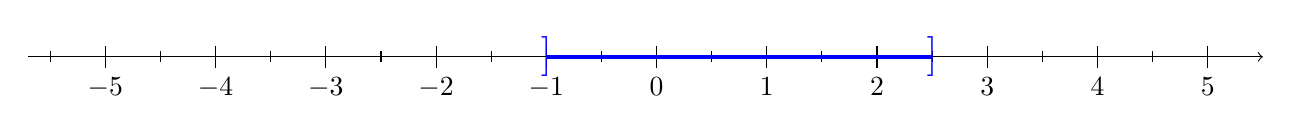
\begin{tikzpicture}[scale=1.4]
    \draw[->] (-5.7,0)--(5.5,0);
    \foreach \x in {-5,..., 5}{
        \draw (\x,0.1)--(\x,-0.1) node[below] {\(\x\)};
        \draw (\x-0.5,0.05)--(\x-0.5,-0.05);
    }
    \draw[blue, ultra thick] (-1,0)--(2.5,0);
    \node[blue] at (-1,0) {\Large \(]\)};
    \node[blue] at (2.5,0) {\Large \(]\)};
    \end{tikzpicture}
    \end{center}
    \item \(\left]-1\ ;\ \dfrac{5}{2}\right]\).
\end{enumerate}
\end{corr}

\begin{corr}{11}
\begin{tasks}(3)
    \task \(]-\infty\ ;\ 4[\)
    \task \([-1\ ;\ +\infty[\)
    \task \(]0\ ;\ 3]\)
    \task \(\left[-2\ ;\ \dfrac{1}{2}\right[\)
    \task \(\left]-\infty\ ;\ -\dfrac{3}{4}\right]\)
    \task \(]2\ ;\ 5[\)
\end{tasks}
Pour la dernière, \(5>x>2\) signifie \(2<x<5\).
\end{corr}

\begin{corr}{12}
Plusieurs réponses sont possibles. Il suffit de vérifier en remplaçant \(x\) par la valeur demandée.
\begin{enumerate}[leftmargin=*]
    \item Par exemple : \(x+3=0\) ; \(2x=-6\) ; \(x-1=-4\).
    \item Par exemple : \(4x=3\), car \(4\times\dfrac{3}{4}=3\).
    \item Par exemple : \(3x=1\), dont la solution est \(\dfrac{1}{3}=0,333\ldots\), qui n'est pas un nombre décimal.
\end{enumerate}
\end{corr}

%%%%%%%%%%%%%%%%%%%%%%%%%%%%%%%%%%%%%%%%%%%%%%%%%%%%%%%%%%%%%%%%%%%%%%%%%%%%%
\section{Fonctions : image, antécédent, représentation graphique}

\begin{corr}[Calculs de début de cours]{13}
\begin{tasks}(3)
    \task \(3x+12\)
    \task \(-2x+10\)
    \task \(-4+x=x-4\)
    \task \(10x-5-3x=7x-5\)
    \task \(x^2+3x\)
    \task \(8x-12\)
\end{tasks}
\end{corr}

\begin{corr}[Guidé]{14}
\begin{enumerate}[leftmargin=*]
    \item \(f(2)=2^2-2\times 2-1=4-4-1=-1\).
    \item \(f(-1)=(-1)^2-2\times(-1)-1=1+2-1=2\).
    \item Tableau de valeurs complété :
    \begin{center}
    \renewcommand{\arraystretch}{2}
    \begin{tabular}{|*{8}{c|}}
        \hline
        \(x\) & \(-1\) & \(-\dfrac{1}{2}\) & \(0\) & \(1\) & \(2\) & \(\dfrac{5}{2}\) & \(3\) \\
        \hline
        \(f(x)\) & \(2\) & \(\dfrac{1}{4}\) & \(-1\) & \(-2\) & \(-1\) & \(\dfrac{1}{4}\) & \(2\) \\
        \hline
    \end{tabular}
    \end{center}
    Par exemple : \(f\left(-\dfrac{1}{2}\right)=\dfrac{1}{4}-2\times\left(-\dfrac{1}{2}\right)-1=\dfrac{1}{4}+1-1=\dfrac{1}{4}\).
    \item Points placés et courbe \(\mathcal{C}_f\) :
    \begin{center}
    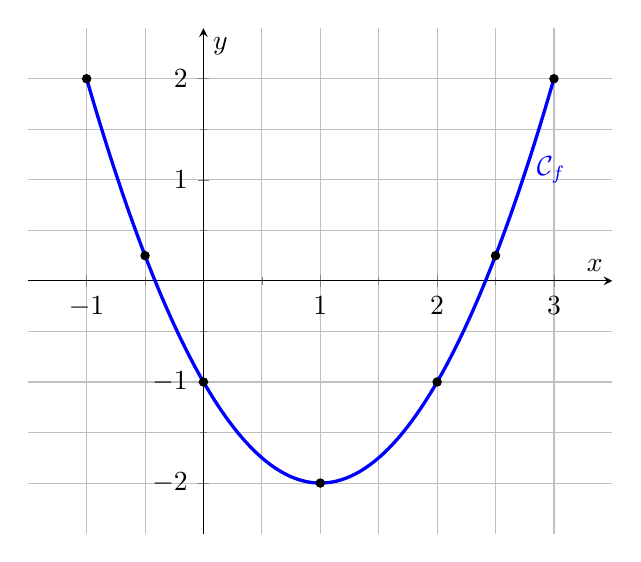
\begin{tikzpicture}
    \begin{axis}[
        axis lines=middle,
        xmin=-1.5, xmax=3.5,
        ymin=-2.5, ymax=2.5,
        grid=both,
        minor tick num=1,
        xtick={-1,0,...,3},
        ytick={-2,-1,...,2},
        xlabel={\(x\)},
        ylabel={\(y\)},
        width=9cm,
        height=8cm
    ]
    \addplot[blue, very thick, domain=-1:3, samples=100] {x^2-2*x-1} node[pos=0.9, right] {\(\mathcal{C}_f\)};
    \addplot[only marks, mark=*, mark size=1.5pt] coordinates {(-1,2)(-0.5,0.25)(0,-1)(1,-2)(2,-1)(2.5,0.25)(3,2)};
    \end{axis}
    \end{tikzpicture}
    \end{center}
    \item \(f(1)=1-2-1=-2\) : le point \(A(1\ ;\ -2)\) appartient à \(\mathcal{C}_f\).

    \(f(3)=9-6-1=2\neq 1\) : le point \(B(3\ ;\ 1)\) n'appartient pas à \(\mathcal{C}_f\).
\end{enumerate}
\end{corr}

\begin{corr}{15}
\begin{enumerate}[leftmargin=*]
    \item \(\mathcal{D}_f=[-3\ ;\ 4]\).
    \item \(f(-2)=3\) ; \(f(0)=0\) ; \(f(2)=0\).
    \item Les antécédents de \(0\) sont \(0\) et \(2\). Le nombre \(-2\) n'a pas d'antécédent : la courbe ne descend jamais jusqu'à l'ordonnée \(-2\).
    \item Les solutions de \(f(x)=2\) sont \(-3\) ; \(-1\) et environ \(3,5\).
    \item Les solutions de \(f(x)=3\) sont \(-2\) et \(4\).
\end{enumerate}
\end{corr}

\begin{corr}{16}
\begin{enumerate}[leftmargin=*]
    \item L'image de \(0\) est \(\dfrac{5}{2}\) ; \(g(-1)=0\).
    \item D'après le tableau, les antécédents de \(4\) sont \(-3\) et \(2\) ; ceux de \(-1\) sont \(-2\) et \(1\).
    \item \(g(3)=\dfrac{1}{2}\), donc \(3\) est une solution de l'équation \(g(x)=\dfrac{1}{2}\).
    \item Non : le tableau ne donne que quelques valeurs, et \(1,5\) n'en fait pas partie. On ne connaît pas l'expression de \(g\).
\end{enumerate}
\end{corr}

\begin{corr}[Vrai ou faux]{17}
\begin{enumerate}[leftmargin=*]
    \item Faux : par définition, une fonction associe à chaque nombre \textbf{une seule} image.
    \item Vrai : \(f(3)=5\) signifie que \(5\) est l'image de \(3\), donc que \(3\) est un antécédent de \(5\).
    \item Faux : un nombre peut avoir plusieurs antécédents. Dans l'exercice 15, \(0\) et \(2\) ont la même image \(0\).
    \item Faux : \(h(2)=\dfrac{2}{2-2}=\dfrac{2}{0}\), et la division par \(0\) est impossible. Le nombre \(2\) n'a pas d'image par \(h\).
\end{enumerate}
\end{corr}

%%%%%%%%%%%%%%%%%%%%%%%%%%%%%%%%%%%%%%%%%%%%%%%%%%%%%%%%%%%%%%%%%%%%%%%%%%%%%
\section{Problèmes}

\begin{corr}[Un rectangle]{18}
\begin{enumerate}[leftmargin=*]
    \item \(P(x)=2(2x+3)+2x=4x+6+2x=6x+6\).
    \item Tableau de valeurs complété :
    \begin{center}
    \renewcommand{\arraystretch}{1.5}
    \begin{tabular}{|*{6}{c|}}
        \hline
        \(x\) & \(1\) & \(2\) & \(3\) & \(4\) & \(5\) \\ \hline
        \(P(x)\) & \(12\) & \(18\) & \(24\) & \(30\) & \(36\) \\ \hline
    \end{tabular}
    \end{center}
    \item
    \(\begin{aligned}[t]
    6x+6 &= 30\\
    6x+6\textcolor{teal}{-6} &= 30\textcolor{teal}{-6}\\
    6x &= 24\\
    x &= 4
    \end{aligned}\)

    Le périmètre du rectangle est égal à \(30\) cm lorsque sa largeur vaut \(4\) cm (on le retrouve dans le tableau).
    \item Pour \(x=4\) : longueur \(2\times 4+3=11\) cm, largeur \(4\) cm. Aire : \(11\times 4=44\) cm\(^2\).
\end{enumerate}
\end{corr}

\begin{corr}[Deux formules d'abonnement]{19}
\begin{enumerate}[leftmargin=*]
    \item \(B(3)=4\times 3+6=18\) et \(B(8)=4\times 8+6=38\). Avec la formule B, \(3\) séances coûtent \(18\) \euro{} et \(8\) séances coûtent \(38\) \euro.
    \item Tableau de valeurs complété :
    \begin{center}
    \renewcommand{\arraystretch}{1.5}
    \begin{tabular}{|*{7}{c|}}
        \hline
        \(x\) & \(0\) & \(2\) & \(4\) & \(6\) & \(8\) & \(10\) \\ \hline
        \(B(x)\) & \(6\) & \(14\) & \(22\) & \(30\) & \(38\) & \(46\) \\ \hline
    \end{tabular}
    \end{center}
    \item \(4x+6=30 \iff 4x=24 \iff x=6\). Pour \(6\) séances, les deux formules coûtent le même prix, \(30\) \euro.
    \item D'après le tableau, le prix de la formule B augmente avec le nombre de séances et vaut \(30\) \euro{} pour \(6\) séances. La formule B est donc la plus avantageuse pour moins de \(6\) séances.
    \item \begin{enumerate}
        \item Réduction : \(\dfrac{15}{100}\times 30=4,5\) \euro. Nouveau prix : \(30-4,5=25,5\) \euro.
        \item \(B(5)=4\times 5+6=26\) \euro{} et \(26>25,5\) : pour \(5\) séances, il vaut mieux choisir la formule A en septembre.
    \end{enumerate}
\end{enumerate}
\end{corr}

\end{document}
